\chapter{RoCEv2的ClickNP实现}
\section{对RoCEv2协议进行抓包分析}
为了充分了解RoCEv2协议,我们利用微软亚洲研究院程鹏研究员基于NetDirect开发的ndping、ndrping工具发送RoCEv2包,
并使用IbDump工具对其进行抓包,用Wireshark进行分析。
\begin{figure}[htbp]
\centering
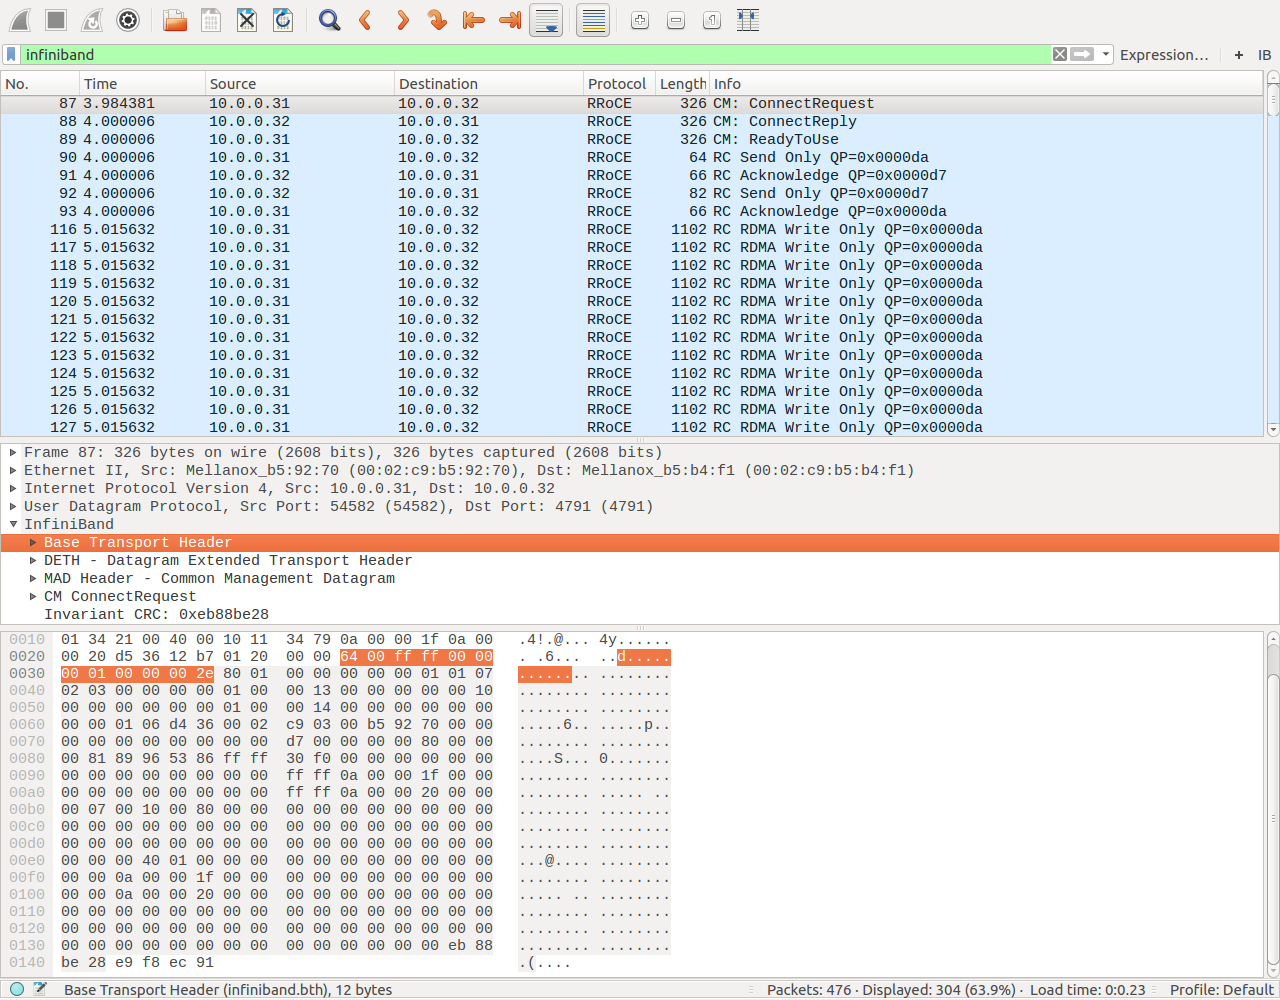
\includegraphics[width=4in]{capture}
\caption{利用Wireshark抓包分析} \label{fig:capture}
\end{figure}

\lstinputlisting[float, floatplacement=htbp, caption=丢包器的ClickNP实现, label=code:drop]{code/PacketDrop.cl}

我们的实验在与同一交换机相连的两台服务器之间进行,期间基本不存在丢包的情况,
所以初期我们只能抓到无丢包情况下的包。

为了解决这一问题,我基于ClickNP平台开发了丢包器,能够在用户的控制下,以一定的概率丢包。
将丢包逻辑写入FPGA,将服务器与交换机之间用FPGA串联,即可通过FPGA将包拦截并丢弃。

将丢包率调整为10\%左右时,可以较好地观察到丢包与重传时所发的包。

在抓包的过程中,我们发现一些根据协议本应出现的包没有被观察到,
例如接收端检测到丢包后会反馈包缺失,而该包在发送端日志中没有体现,
但发送端的重传行为就好像收到了这样的反馈。我们据此猜测IbDump没有将流经网卡的包全部记录下来。

为了验证这一猜测,我们改在FPGA上抓包。在丢包器的下游增设抓包器,在记录包的同时将其发出。

在使用FPGA抓包的过程中,我们发现当发包频率加快时,会出现阻塞情况。
这是因为抓包器将包记录在主机上需要通过PCIe接口发送数据,
而PCIe接口的数据带宽低于FPGA网卡的带宽,因此缓冲区会被迅速写满,随后不再响应网卡的输入请求。

为了解决这一问题,我对ndping、ndrping的代码进行了修改,将原有的连续发送RDMA请求改为有时间间隔地发送RDMA请求。
虽然在请求长度较大时仍然会出现阻塞情况,但因为我们在FPGA上的抓包实验侧重于对丢包情况进行分析,
因此不需要发送长度太大的RDMA请求。

实验表明,FPGA的抓包结果中确实出现了之前IbDump没有记录下来的包,
这证实了我们的猜测,也验证了我们对于RoCEv2协议的初步理解。

在IbDump与FPGA两个抓包工具获取到的日志基础上进行分析,使我们加深了对RoCEv2协议的认识。

\section{项目实现}
RoCEv2项目包含如下元件:
\begin{figure}[htbp]
\centering
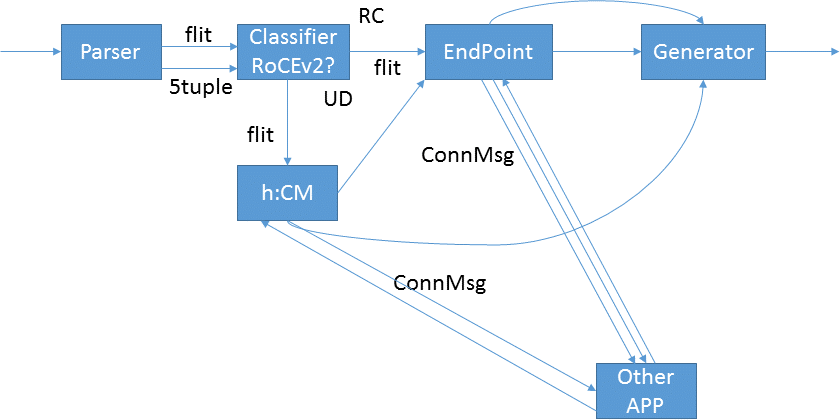
\includegraphics[width=4in]{roce}
\caption{RoCEv2各元件及其连接关系} \label{fig:roce}
\note{红框内为我们项目的实现细节,对应用程序是透明的。}
\end{figure}

\lstinputlisting[float, floatplacement=htbp, caption=RoCEv2项目的ClickNP配置文件, label=code:rocecfg]{code/RoCE.cfg}

\begin{figure}[htbp]
\centering
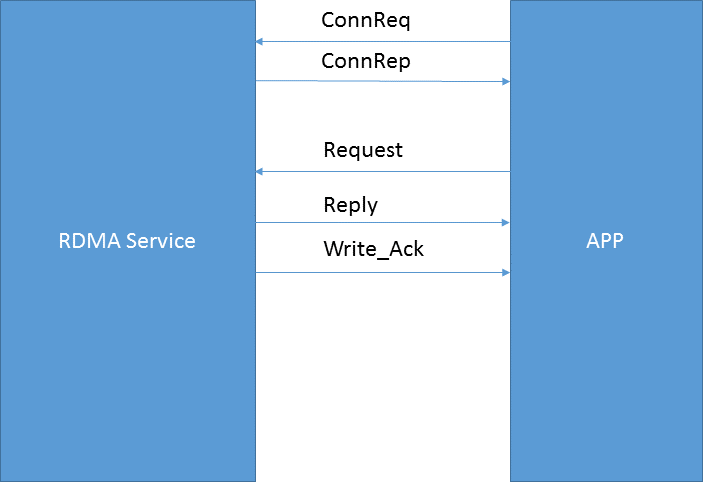
\includegraphics[width=4in]{roceapi}
\caption{应用程序与适配器之间的5条通道} \label{fig:roceapi}
\end{figure}

\begin{description}
\item[RoCE\_Classifier包分类器]将收到的包进行分类,将连接相关请求转发至连接管理器,将数据请求转发至适配器。
\item[RoCE\_Connector连接管理器]根据连接请求,建立、维护、断开连接。
\item[应用程序]向终端发起应用RDMA请求。
\item[RoCE\_Endpoint终端]与应用程序交互,将用户的请求转发至包生成器,并向应用程序发送反馈。
\item[RoCE\_Gen包生成器]将连接管理器和终端发来的请求翻译为网络协议包。
\end{description}

图~\ref{fig:roce} 展示各元件间的连接关系,其配置文件如代码~\ref{code:rocecfg} 所示。

应用程序与适配器之间的5条通道功能如图~\ref{fig:roceapi} 所示。

我在该项目中负责实现包生成器。该器件有2个输入端口和1个输出端口。
其中输入端口1与终端相连,输入端口2与连接管理器相连;输出端口与网卡相连。
当输入端口有收到发包请求时,包生成器根据收到的元数据填写待发送帧的各个域,
并维护其操作码及序列号两个状态,每周期处理一帧,直到最后一帧发送完毕,读取下一个请求。

在该协议的实现中,终端和连接管理器向包生成器发送的元数据帧信息量总是足以供包生成器填充等量要发送的帧。
所以只要输入端有源源不断的发包请求,包生成器在每个周期就都会有帧输出。
不需要手工维护多级流水线及其缓冲区即可充分利用设备的吞吐率。

包生成器的大致框架如代码~\ref{code:rocegen} 所示。
截至我从微软亚洲研究院离职时,包生成器已实现CM ConnectionReply、CM ReadyToUse、
Acknowledge、RC RDMA Read Request等功能,代码量不足八百行,
预计实现全部功能只需要四千行代码。

另外,看似比较大的代码量不代表程序效率低下。因为同一个分支内不存在数据依赖,
所以这些代码在FPGA中很容易实现并行化,可以认为是同时执行。

\newpage
\lstinputlisting[caption=RoCE\_Gen包生成器示意,label=code:rocegen]{code/RoCE_Gen.cl}
